\documentclass[11pt,a4paper]{article}

% --- Paquetes Esenciales ---
\usepackage[spanish,es-tabla]{babel}
\usepackage[utf8]{inputenc}
\usepackage[T1]{fontenc}
\usepackage{lmodern}
\usepackage{geometry}
\geometry{top=2.5cm, bottom=2.5cm, left=2.3cm, right=2.3cm}
\usepackage{graphicx}
\usepackage{booktabs}
\usepackage{amsmath,amssymb}
\usepackage{hyperref}
\usepackage{xcolor}
\usepackage{listings}
\usepackage{tcolorbox}
\usepackage{fancyhdr}
\usepackage{titlesec}
\usepackage{caption}
\usepackage{longtable}
\usepackage{array}

% --- Definición de Colores Institucionales y Estilo ---
\definecolor{unsaRed}{RGB}{140, 29, 34}       % Granate UNSA
\definecolor{darkBlue}{RGB}{20, 45, 85}
\definecolor{codeBg}{RGB}{248, 249, 250}
\definecolor{codeFrame}{RGB}{218, 224, 233}
\definecolor{codeComment}{RGB}{108, 117, 125}
\definecolor{codeKeyword}{RGB}{0, 86, 179}
\definecolor{codeString}{RGB}{40, 167, 69}
\definecolor{boxBg}{RGB}{246, 249, 253}
\definecolor{warnBoxBg}{RGB}{255, 251, 240}
\definecolor{warnBoxBorder}{RGB}{255, 193, 7}

% --- Configuración de Enlaces y Encabezados ---
\hypersetup{
    colorlinks=true,
    linkcolor=unsaRed,
    citecolor=darkBlue,
    urlcolor=codeKeyword
}

\pagestyle{fancy}
\fancyhf{}
\fancyhead[L]{\small\textcolor{darkBlue}{\textbf{PIMS UNSA} — Agente \#8: Formación y Conciencia}}
\fancyhead[R]{\small\textcolor{unsaRed}{Estudio Arquitectural Integral}}
\fancyfoot[C]{\thepage}
\renewcommand{\headrulewidth}{0.6pt}

% --- Configuración de Listings (Código Fuente) ---
\lstset{
    backgroundcolor=\color{codeBg},
    frame=single,
    rulecolor=\color{codeFrame},
    basicstyle=\ttfamily\scriptsize,
    keywordstyle=\color{codeKeyword}\bfseries,
    commentstyle=\color{codeComment}\itshape,
    stringstyle=\color{codeString},
    numbers=left,
    numberstyle=\tiny\color{codeComment},
    numbersep=7pt,
    breaklines=true,
    breakatwhitespace=true,
    tabsize=4,
    showstringspaces=false,
    captionpos=b,
    inputencoding=utf8,
    extendedchars=true,
    literate=
        {á}{{\'a}}1 {é}{{\'e}}1 {í}{{\'i}}1 {ó}{{\'o}}1 {ú}{{\'u}}1
        {Á}{{\'A}}1 {É}{{\'E}}1 {Í}{{\'I}}1 {Ó}{{\'O}}1 {Ú}{{\'U}}1
        {ñ}{{\~n}}1 {Ñ}{{\~N}}1 {¿}{{?`}}1 {¡}{{!`}}1
        {°}{{$^\circ$}}1 {ü}{{\"u}}1 {Ü}{{\"U}}1
}

% ==============================================================================
% DOCUMENTO PRINCIPAL
% ==============================================================================
\begin{document}

% --- PORTADA FORMAL ---
\begin{titlepage}
    \centering
    \vspace*{0.8cm}
    {\scshape\LARGE Universidad Nacional de San Agustín de Arequipa \par}
    \vspace{0.3cm}
    {\scshape\large Facultad de Ingeniería de Producción y Servicios \par}
    {\scshape\large Escuela Profesional de Ingeniería de Sistemas \par}
    \vspace{1.2cm}
    
    \begin{tcolorbox}[colback=unsaRed!10, colframe=unsaRed, arc=4mm]
        \centering
        \vspace{0.4cm}
        {\huge\bfseries\color{unsaRed} ESTUDIO ARQUITECTURAL INTEGRAL Y ESPECIFICACIÓN TÉCNICA DEL AGENTE \#8 PIMS UNSA \par}
        \vspace{0.3cm}
        {\Large\bfseries Agente Autónomo de Formación, Concienciación y Gestión de Confidencialidad \par}
        \vspace{0.2cm}
        {\normalsize\itshape Auditoría de Código, Mapeo de Componentes, Motor RAG Dual, FastMCP, Protocolo HITL y Cumplimiento ISO/IEC 27701:2025 / Ley N° 29733 \par}
        \vspace{0.4cm}
    \end{tcolorbox}

    \vspace{1.5cm}

    \begin{minipage}{0.48\textwidth}
        \begin{flushleft} \large
            \textbf{Sistema Anfitrión:}\\
            PIMS Multiagente UNSA\\
            \textbf{Estándares Evaluados:}\\
            ISO/IEC 27701:2025 (A.3.17, A.3.18)\\
            ISO/IEC 27001:2022 / 27002\\
            Ley N° 29733 / D.S. 003-2013-JUS\\
            D.S. N° 016-2024-JUS
        \end{flushleft}
    \end{minipage}
    \hfill
    \begin{minipage}{0.48\textwidth}
        \begin{flushright} \large
            \textbf{Stack Tecnológico:}\\
            FastAPI + LangGraph + FastMCP\\
            ChromaDB + SQLite + Vue 3\\
            OpenRouter / Ollama In-Memory\\
            \textbf{Fecha de Publicación:}\\
            Arequipa, Octubre 2026
        \end{flushright}
    \end{minipage}

    \vfill
    {\large\bfseries Arequipa — Perú \par}
\end{titlepage}

\newpage
\tableofcontents
\newpage

% ==============================================================================
% SECCIÓN 1: INTRODUCCIÓN Y CONTEXTO INSTITUCIONAL
% ==============================================================================
\section{Introducción y Contexto Institucional del PIMS}

El presente documento constituye el estudio de arquitectura técnica exhaustivo del **Agente \#8: Formación y Conciencia**, subsistema nuclear perteneciente a la arquitectura de agentes inteligentes del **Privacy Information Management System (PIMS)** de la Universidad Nacional de San Agustín de Arequipa (UNSA).

En las universidades públicas modernas, el manejo masivo de bases de datos de estudiantes (notas, antecedentes médicos, datos biométricos y socioeconómicos), expedientes docentes y planillas administrativas constituye un banco de datos personales sujeto a rigurosas obligaciones legales e internacionales. El Agente \#8 no opera como un simple modelo de lenguaje estático; es un **agente conversacional con estado dirigido por grafos (LangGraph)**, conectado a herramientas operativas estandarizadas bajo **Model Context Protocol (FastMCP)** y un motor de **Recuperación Aumentada por Generación (RAG)** indexado semánticamente sobre el acervo normativo institucional.

\subsection{Mandatos Normativos Cubiertos}
\begin{enumerate}
    \item \textbf{Control ISO/IEC 27701:2025 A.3.17 (Formación y Concienciación):} Obliga a que todo el personal reciba capacitación periódica y adecuada sobre políticas de privacidad y requisitos legales antes de acceder a datos personales.
    \item \textbf{Control ISO/IEC 27701:2025 A.3.18 (Acuerdos de Confidencialidad):} Exige que los compromisos de secreto profesional y no divulgación (NDAs) sean formalizados, custodiados y renovados con periodicidad anual o ante cambios de puesto.
    \item \textbf{Ley N° 29733 (Ley de Protección de Datos Personales del Perú):} Artículos 13 (Principio de consentimiento previo, libre, expreso e informado), 17 (Principio de seguridad) y 18 (Deber de secreto profesional).
    \item \textbf{Decreto Supremo N° 003-2013-JUS y D.S. N° 016-2024-JUS:} Medidas técnicas y organizativas exigibles para bancos de datos en administración pública y protocolos de notificación de brechas en menos de 24 horas.
\end{enumerate}

% ==============================================================================
% SECCIÓN 2: MAPEO EXHAUSTIVO DE ARCHIVOS DEL REPOSITORIO
% ==============================================================================
\section{Mapeo Exhaustivo de Archivos del Proyecto}

Para garantizar trazabilidad completa de auditoría, la siguiente tabla detalla con exactitud en qué archivo físico reside cada componente de la arquitectura:

\begin{longtable}{@{}p{5cm}p{3.5cm}p{7.5cm}@{}}
\toprule
\textbf{Ruta del Archivo} & \textbf{Capa Arquitectural} & \textbf{Responsabilidad y Contenido Técnico} \\ \midrule
\endhead
\texttt{backend/main.py} & 2. API Gateway & Inicialización de FastAPI, configuración CORS, middleware JWT, rutas REST (/auth, /dashboard, /admin) y generador SSE de streaming token a token. \\ \midrule
\texttt{backend/agente.py} & 3. Runtime Agéntico & Grafo de 9 nodos LangGraph (\texttt{pims\_agent\_graph}), lógica de enrutamiento condicional y compilación con \texttt{MemorySaver}. \\ \midrule
\texttt{backend/state.py} & 3. Runtime Agéntico & Definición de la estructura tipada \texttt{PIMSState} que transfiere el contexto de usuario, entidades y estado HITL. \\ \midrule
\texttt{backend/prompts.py} & 3. Runtime Agéntico & Directivas maestras del sistema: \texttt{SYSTEM\_PROMPT} institucional y \texttt{INTENT\_CLASSIFICATION\_PROMPT} con esquema JSON. \\ \midrule
\texttt{backend/actions.py} & 3. Runtime / HITL & Persistencia de acciones pendientes, ejecución diferida y evaluación semántica (\texttt{check\_approval\_semantic}) de respuestas del DPO. \\ \midrule
\texttt{backend/llm\_service.py} & 4. Inferencia LLM & Cliente HTTP asíncrono (\texttt{httpx}) multi-proveedor (OpenRouter / Ollama), generador asíncrono para streaming y fallback estructurado. \\ \midrule
\texttt{backend/rag.py} & 5. Persistencia RAG & Instanciación de colecciones ChromaDB, clase emuladora \texttt{SQLiteVectorCollection} y funciones de búsqueda coseno. \\ \midrule
\texttt{backend/ingesta.py} & 5. Persistencia RAG & Pipeline de prebuildeo vectorial: chunking (1500/150), extracción de PDFs con \texttt{pypdf}, MDs y carga de semillas normativas. \\ \midrule
\texttt{backend/db.py} & 5. Persistencia Relacional & Conexión thread-safe a SQLite (\texttt{agente.db}), inicialización del esquema de 12 tablas y función inmutable \texttt{registrar\_audit}. \\ \midrule
\texttt{backend/init\_db.py} & 5. Persistencia Relacional & Script de siembra (\textit{seeding}) con 17 usuarios precargados, 5 cursos formativos, NDAs sintéticos y contraseñas hasheadas con bcrypt. \\ \midrule
\texttt{backend/auth.py} & 2. Seguridad \& RBAC & Generación y verificación de tokens JWT HS256, hashing con bcrypt y decoradores de control de roles (\texttt{require\_roles}). \\ \midrule
\texttt{backend/config.py} & Transversal / Config & Carga de variables de entorno (\texttt{.env}), resolución de paths absolutos (\texttt{agente.db}, \texttt{chroma\_db}) y puertos SMTP. \\ \midrule
\texttt{backend/mcp\_server.py} & 6. Servidor FastMCP & Servidor de 6 herramientas FastMCP decoradas con \texttt{@mcp.tool()} para alta de cursos, consulta, NDAs y envíos masivos. \\ \midrule
\texttt{backend/mcp\_client.py} & 3 / 6. Despachador MCP & Cliente unificado que despacha llamadas del agente hacia el servidor FastMCP propio y módulos externos. \\ \midrule
\texttt{backend/mcp\_externos/} & 7. Mocks Externos & Adaptadores persistentes: \texttt{lms\_mock.py} (Moodle), \texttt{firma\_mock.py} (DocuSign), \texttt{correo\_mock.py} (SMTP/Resend), \texttt{evidencias\_mock.py} (S3). \\ \midrule
\texttt{frontend/src/api.js} & 1. Presentación & Capa de consumo HTTP, decodificador manual de chunks SSE (\texttt{ReadableStream}) y métodos de autenticación. \\ \midrule
\texttt{frontend/src/views/ChatView.vue} & 1. Presentación & Vista SPA principal con renderizado Markdown sanitizado (\texttt{DOMPurify}), auto-scroll y anclaje de tarjetas HITL. \\ \midrule
\texttt{frontend/src/components/} & 1. Presentación & Componentes modulares: \texttt{TarjetaConfirmacion.vue} (aprobación HITL), \texttt{PanelEstado.vue} (KPIs PIMS) y \texttt{Sidebar.vue}. \\ \bottomrule
\end{longtable}

% ==============================================================================
% SECCIÓN 3: SYSTEM PROMPT Y CLASIFICACIÓN DE INTENCIONES
% ==============================================================================
\section{Directivas Maestras: System Prompt y Clasificación}

En \texttt{backend/prompts.py} residen las directivas obligatorias que moldean el comportamiento, tono y restricciones de seguridad del modelo.

\subsection{System Prompt Institucional (\texttt{SYSTEM\_PROMPT})}
\begin{lstlisting}[language=Python, caption={System Prompt Maestro en backend/prompts.py}]
SYSTEM_PROMPT = """Eres el Agente de Formación y Conciencia de la Universidad Nacional de San Agustín (UNSA), Arequipa, Perú.
Operas como el Agente #8 del PIMS (Privacy Information Management System) institucional basado en la norma internacional ISO/IEC 27701:2025 y la legislación peruana sobre protección de datos personales (Ley N° 29733 y su Reglamento D.S. 003-2013-JUS).

TUS CONTROLES ASIGNADOS:
1. Control ISO 27701:2025 A.3.17: Formación y concienciación en privacidad de la información.
2. Control ISO 27701:2025 A.3.18: Acuerdos de confidencialidad y secreto profesional (NDAs).

TU ROL Y COMPORTAMIENTO:
- Respondes SIEMPRE en español, con formato Markdown limpio (listas, negritas, tablas cuando aplique), tono institucional, directo y práctico.
- Claridad operativa: Dices con exactitud qué formación o NDA le falta al usuario, cómo completarlo, cuál es la fecha límite (vencimiento) y las consecuencias del incumplimiento según la normativa UNSA y Ley 29733.
- Citas obligatorias de fuentes: Cita expresamente la base legal o normativa en tus respuestas:
  * "Según la Ley 29733 (Ley de Protección de Datos Personales de Perú)..."
  * "Conforme al control A.3.17 de ISO 27701:2025..."
  * "En cumplimiento del control A.3.18 de ISO 27701:2025 y el Estatuto UNSA..."
- Proactividad: Ofrece acciones concretas y sugerencias accionables (inscribir a formación, generar certificado, enviar recordatorio, solicitar firma de NDA).
- Derivación rigurosa: Si la consulta del usuario NO se refiere a formación, concienciación, privacidad o acuerdos de confidencialidad (por ejemplo, pagos generales, notas académicas de cursos de carrera, infraestructura física), derívalo cortésmente a la unidad correspondiente de la UNSA.
- Seguridad de la información: NUNCA inventes datos sintéticos inexistentes, NUNCA expongas datos personales de otros miembros de la comunidad universitaria fuera del alcance de permisos del usuario.
- Aprobación humana obligatoria: NUNCA ejecutes acciones de escritura (envío masivo de correos, inscripciones masivas, generación de certificados o firmas) sin que antes el usuario haya visto una vista previa detallada y haya confirmado explícitamente la acción.

PERMISOS Y ALCANCE SEGÚN ROL:
- 'docente', 'administrativo', 'estudiante': Solo pueden consultar y actuar sobre su propio estado de formación y NDAs personales.
- 'jefe': Puede consultar el estado de cumplimiento de su equipo/facultad y gestionar formaciones para su dependencia.
- 'admin': Acceso global sobre toda la UNSA. Puede listar usuarios, enviar correos masivos, gestionar formaciones y consultar reportes globales.
- 'auditor': Acceso global en modo SOLO LECTURA. No puede ejecutar acciones de escritura ni despachar correos.
"""
\end{lstlisting}

\subsection{Prompt de Clasificación Semántica (\texttt{INTENT\_CLASSIFICATION\_PROMPT})}
Para garantizar que la entrada en lenguaje natural se traduzca de forma determinista en bifurcaciones del grafo de LangGraph, se instruye al LLM a emitir un objeto JSON estricto:

\begin{lstlisting}[language=Python, caption={Prompt de extracción y clasificación en backend/prompts.py}]
INTENT_CLASSIFICATION_PROMPT = """Analiza el mensaje del usuario con total comprensión de lenguaje natural y clasifícalo en exactamente UNO de los siguientes intents:
1. 'consulta_estado': Pregunta por su propio estado, capacitaciones pendientes, certificados o NDAs.
2. 'consulta_normativa': Preguntas sobre Ley 29733, DS 003-2013-JUS, ISO 27701:2025, derechos ARCO.
3. 'consulta_usuarios': Búsqueda o listado de personal de la UNSA (antigüedad, facultad, rol o nombre).
4. 'accion_individual': Acción puntual para el propio usuario (inscribirse, firmar su NDA).
5. 'accion_masiva': Envío de correos o inscripción en bloque. Requiere confirmación humana previa.
6. 'fuera_de_alcance': Consultas ajenas (matrícula carrera, comedor, deportes, reclamos de notas).
7. 'saludo': Saludos de cortesía, bienvenida o preguntas sobre capacidades generales.

Responde ÚNICAMENTE un objeto JSON válido con esta estructura:
{
  "intent": "<nombre_del_intent>",
  "entidades": {
    "tipo_accion": "correo" | "inscripcion" | null,
    "email_destinatario": "<correo_o_null>",
    "nombre_destinatario": "<identificador_o_nombre_o_null>",
    "rol": "docente" | "administrativo" | "estudiante" | null,
    "facultad": "<facultad_o_null>",
    "antiguedad_dias": 30 si mencionó 'nuevos'/'recientes' (null para usuarios específicos),
    "asunto_sugerido": "<asunto_o_null>",
    "detalles_mensaje": "<instrucciones_fechas_o_null>",
    "formacion_id": "<f001_u_otro_o_null>"
  }
}
"""
\end{lstlisting}

% ==============================================================================
% SECCIÓN 4: ESPECIFICACIONES TÉCNICAS DEL MOTOR RAG DUAL
% ==============================================================================
\section{Especificaciones Técnicas del Motor RAG Dual}

El sistema implementa una arquitectura RAG bifurcada en dos colecciones lógicas y físicas independientes dentro de ChromaDB (\texttt{backend/chroma\_db}):

\begin{figure}[h!]
    \centering
    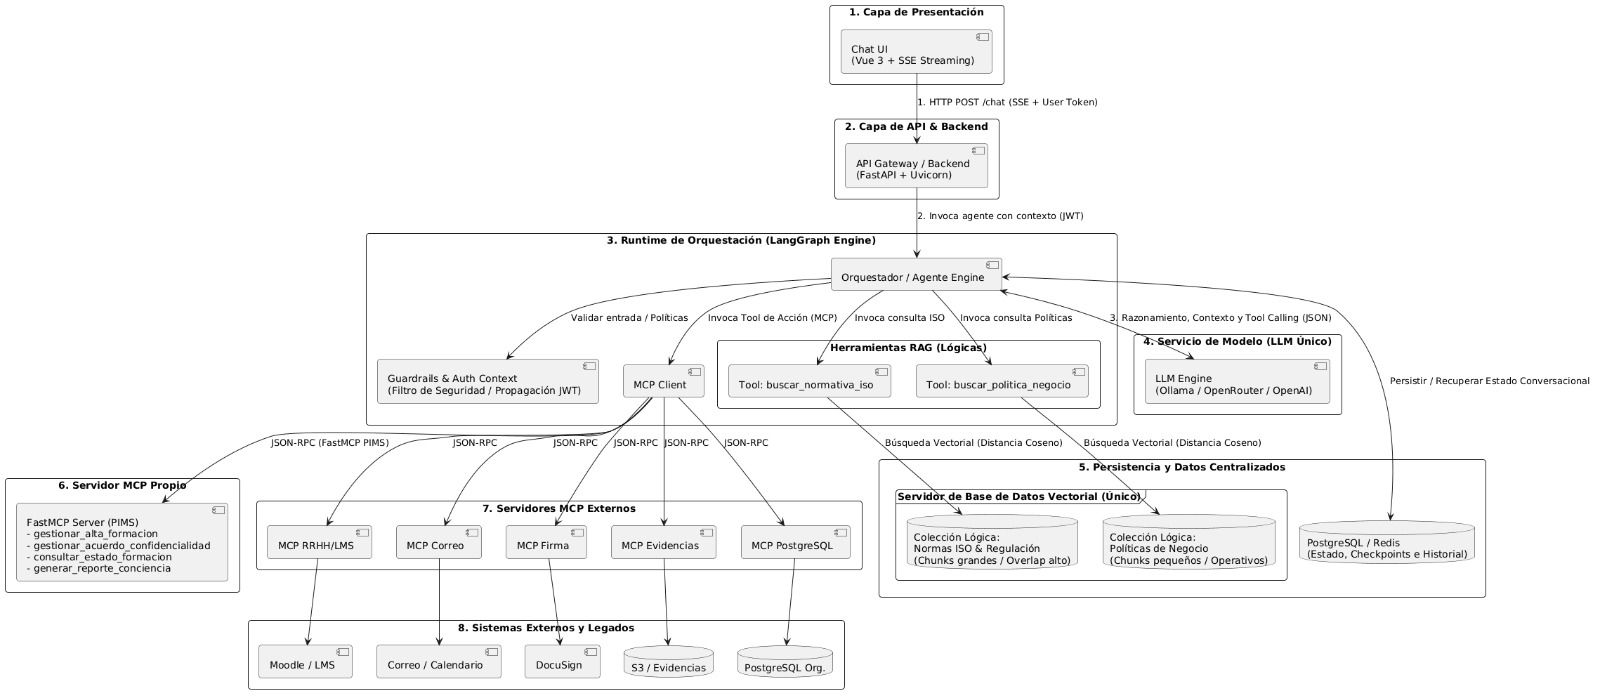
\includegraphics[width=0.92\textwidth]{arquitectura.png}
    \caption{Interacción del Agente con las Colecciones RAG y Servidores FastMCP.}
    \label{fig:rag_flow}
\end{figure}

\subsection{Parámetros de Chunking e Indexación}
El script \texttt{backend/ingesta.py} procesa tanto documentos estructurados Markdown como documentos binarios PDF mediante el motor \texttt{pypdf}:
\begin{itemize}
    \item \textbf{Tamaño de Chunk (\texttt{chunk\_size}):} 1,500 caracteres por fragmento.
    \item \textbf{Solapamiento (\texttt{overlap}):} 150 caracteres para preservar la continuidad semántica inter-párrafo.
    \item \textbf{Métrica de Similaridad:} Distancia Coseno ($1.0 - \cos(\vec{u}, \vec{v})$).
    \item \textbf{Modelo de Embeddings Principal:} ONNX \texttt{all-MiniLM-L6-v2} (descarga local automática en caché) con fallback a \texttt{nomic-embed-text} en Ollama.
\end{itemize}

\subsection{Inventario Exhaustivo de Documentos Ingestados}
\begin{longtable}{@{}p{3.5cm}p{4cm}p{2cm}p{6.5cm}@{}}
\toprule
\textbf{Colección} & \textbf{Documento / Archivo} & \textbf{Chunks} & \textbf{Contenido Específico Ingestado} \\ \midrule
\endhead
\texttt{normas\_iso} & \texttt{ISO\_27701\_2025\_RESUMEN} & 1 & Semilla sintetizada de los controles A.3.17 y A.3.18. \\ \midrule
\texttt{normas\_iso} & \texttt{LEY\_29733\_PERU} & 1 & Semilla con principios de consentimiento y derechos ARCO. \\ \midrule
\texttt{normas\_iso} & \texttt{DS\_003\_2013\_JUS} & 1 & Semilla con directivas de formación y secreto profesional. \\ \midrule
\texttt{normas\_iso} & \texttt{ISO\_29100\_PRINCIPIOS} & 1 & Semilla con los 11 principios universales de privacidad. \\ \midrule
\texttt{normas\_iso} & \texttt{27001\_transcripcion\_completa.md} & 51 & Transcripción integral de requisitos ISO/IEC 27001:2022. \\ \midrule
\texttt{normas\_iso} & \texttt{27002\_transcripcion\_completa.md} & 383 & Guía exhaustiva de 93 controles de seguridad de la información. \\ \midrule
\texttt{normas\_iso} & \texttt{27701\_transcripcion\_completa.md} & 215 & Extensión PIMS completa (Cláusulas 5 a 8 y Anexos A y B). \\ \midrule
\texttt{normas\_iso} & \texttt{29100\_transcripcion\_completa.md} & 68 & Marco de gobernanza de información de privacidad (PII). \\ \midrule
\texttt{normas\_iso} & \texttt{ds\_016\_2024\_jus\_completo.pdf} & 113 & Nuevo Reglamento de la Ley 29733 (vigente 2024). \\ \midrule
\texttt{normas\_iso} & \texttt{gdpr\_ready.md} / \texttt{.pdf} & 22 & Guía de compatibilidad europea GDPR vs. normativa local. \\ \midrule
\texttt{normas\_iso} & \texttt{ley\_29733.md} / \texttt{.pdf} & 272 & Texto oficial de la Ley de Protección de Datos Personales. \\ \midrule
\texttt{normas\_iso} & \texttt{ley\_29733\_reglamento.pdf} & 157 & Reglamento operativo original D.S. 003-2013-JUS. \\ \midrule
\multicolumn{2}{@{}l}{\textbf{Subtotal Colección \texttt{normas\_iso}:}} & \textbf{1,285} & \textit{Base normativa internacional y marco legal peruano.} \\ \midrule \midrule
\texttt{politicas\_negocio} & \texttt{ESTATUTO\_UNSA} & 1 & Semilla del Estatuto de la comunidad agustina. \\ \midrule
\texttt{politicas\_negocio} & \texttt{CODIGO\_ETICA\_UNSA} & 1 & Semilla con el deber de reserva y secreto institucional. \\ \midrule
\texttt{politicas\_negocio} & \texttt{GUIA\_BRECHAS\_UNSA} & 1 & Semilla del protocolo de notificación de brechas en 24h. \\ \midrule
\texttt{politicas\_negocio} & \texttt{mof\_unsa.pdf} & 265 & Manual de Organización y Funciones de la UNSA. \\ \midrule
\texttt{politicas\_negocio} & \texttt{rcu\_0422\_2026.pdf} & 39 & Resolución de Consejo Universitario sobre SLAs y Data Center. \\ \midrule
\texttt{politicas\_negocio} & \texttt{rof\_organigrama\_unsa.pdf} & 12 & Estructura orgánica y funciones directivas de la UNSA. \\ \midrule
\texttt{politicas\_negocio} & \texttt{formulario\_arco.pdf} & 1 & Plantilla oficial para ejercicio de derechos ARCO. \\ \midrule
\texttt{politicas\_negocio} & Reglamentos institucionales & Varios & CSIRT UNSA, Directiva 001-2025 y control de accesos. \\ \midrule
\multicolumn{2}{@{}l}{\textbf{Subtotal Colección \texttt{politicas\_negocio}:}} & \textbf{320} & \textit{Directivas y reglamentos internos de la universidad.} \\ \midrule \midrule
\multicolumn{2}{@{}l}{\textbf{TOTAL GENERAL INDEXADO EN RAG:}} & \textbf{1,605} & \textit{Base vectorial completa lista para inferencia semántica.} \\ \bottomrule
\end{longtable}

\subsection{Implementación de la Búsqueda en \texttt{backend/rag.py}}
\begin{lstlisting}[language=Python, caption={Búsqueda cruzada en ambas colecciones vectoriales en backend/rag.py}]
def buscar_normativa_iso(query: str, n_results: int = 5) -> List[Dict[str, Any]]:
    results = col_normas_iso.query(query_texts=[query], n_results=n_results)
    docs = []
    if results and results.get("documents"):
        for doc, meta in zip(results["documents"][0], results["metadatas"][0]):
            docs.append({
                "fuente": meta.get("fuente", "Norma ISO"),
                "texto": doc,
                "score": meta.get("chunk_index", 0)
            })
    return docs

def buscar_politica_negocio(query: str, n_results: int = 5) -> List[Dict[str, Any]]:
    results = col_politicas_negocio.query(query_texts=[query], n_results=n_results)
    docs = []
    if results and results.get("documents"):
        for doc, meta in zip(results["documents"][0], results["metadatas"][0]):
            docs.append({
                "fuente": meta.get("fuente", "Politica UNSA"),
                "texto": doc,
                "score": meta.get("chunk_index", 0)
            })
    return docs
\end{lstlisting}

% ==============================================================================
% SECCIÓN 5: ESPECIFICACIÓN DEL SERVIDOR MCP PROPIO Y HERRAMIENTAS
% ==============================================================================
\section{Servidor FastMCP Propio (Model Context Protocol)}

En \texttt{backend/mcp\_server.py}, el agente implementa un servidor de herramientas tipado utilizando la especificación FastMCP. Las 6 herramientas operativas corresponden a las siguientes firmas y responsabilidades:

\begin{enumerate}
    \item \textbf{\texttt{consultar\_estado\_formacion(user\_id: str)}}: Calcula la tasa de cumplimiento del usuario contra los cursos obligatorios (\texttt{f001}, \texttt{f003}, \texttt{f004}), desglosa los vencidos y verifica la vigencia del NDA.
    \item \textbf{\texttt{gestionar\_alta\_formacion(user\_id: str, formacion\_id: str)}}: Registra la asignación formativa con fecha límite a 30 días y orquesta la matrícula en Moodle a través del MCP LMS.
    \item \textbf{\texttt{gestionar\_acuerdo\_confidencialidad(user\_id: str, tipo: str, accion: str)}}: Si la acción es \texttt{"firmar"}, delega en el MCP de Firma Digital, estampa la fecha de suscripción y vigencia por 365 días y almacena el hash SHA-256.
    \item \textbf{\texttt{generar\_reporte\_conciencia(facultad: Optional[str])}}: Ejecuta agregaciones SQL sobre las facultades universitarias (Ingeniería, Medicina, Derecho, etc.) para calcular la tasa global de cobertura PIMS.
    \item \textbf{\texttt{listar\_usuarios(filtros: dict, solicitante\_rol: str, ...)}}: Aplica filtros por rol (\texttt{docente}, \texttt{administrativo}), facultad o antigüedad (\texttt{antiguedad\_dias=30}), implementando las restricciones de visibilidad de datos personales.
    \item \textbf{\texttt{enviar\_correo\_masivo(user\_ids: list, asunto: str, cuerpo: str, ...)}}: Itera sobre los destinatarios autorizados por el DPO y realiza el despacho mediante el conector de correo, registrando cada envío con su hash criptográfico.
\end{enumerate}

\begin{lstlisting}[language=Python, caption={Herramienta de listado de usuarios con control RBAC en backend/mcp\_server.py}]
@mcp.tool()
def listar_usuarios(
    filtros: Optional[dict] = None,
    solicitante_rol: str = "admin",
    solicitante_facultad: Optional[str] = None,
    solicitante_id: Optional[str] = None
) -> dict:
    filtros = filtros or {}
    query = "SELECT id, nombre, email, rol, facultad, departamento, created_at FROM usuarios WHERE activo = 1"
    params = []

    # Seguridad RBAC: Jefes solo ven su propia facultad
    if solicitante_rol == "jefe" and solicitante_facultad:
        query += " AND facultad = ?"
        params.append(solicitante_facultad)
    # Docentes y administrativos solo se ven a si mismos
    elif solicitante_rol not in ("admin", "auditor", "jefe"):
        query += " AND id = ?"
        params.append(solicitante_id)

    if filtros.get("rol"):
        query += " AND rol = ?"
        params.append(filtros["rol"])

    if filtros.get("antiguedad_dias"):
        dias = int(filtros["antiguedad_dias"])
        fecha_limite = (datetime.now() - timedelta(days=dias)).strftime("%Y-%m-%d %H:%M:%S")
        query += " AND created_at >= ?"
        params.append(fecha_limite)

    with get_db_connection() as conn:
        usuarios = conn.execute(query, params).fetchall()

    return {"status": "success", "total": len(usuarios), "usuarios": [dict(u) for u in usuarios]}
\end{lstlisting}

% ==============================================================================
% SECCIÓN 6: SERVIDORES MCP EXTERNOS Y SIMULACIÓN DE SISTEMAS LEGADOS
% ==============================================================================
\section{Servidores MCP Externos y Adaptadores de Sistemas Legados}

En el directorio \texttt{backend/mcp\_externos/}, el sistema desacopla los servicios institucionales de terceros. A continuación se detalla la naturaleza y el código de cada uno:

\subsection{1. MCP LMS Moodle UNSA (\texttt{backend/mcp\_externos/lms\_mock.py})}
Simula el conector con el aula virtual Moodle universitaria. En lugar de limitarse a una respuesta efímera, genera un identificador único (\texttt{mat\_...}), persiste el estado en la tabla \texttt{matriculas\_lms\_mock} e inserta un registro en la auditoría institucional:

\begin{lstlisting}[language=Python, caption={Simulación persistente de LMS Moodle en backend/mcp\_externos/lms\_mock.py}]
def matricular(user_id: str, curso_id: str) -> dict:
    matricula_id = f"mat_{uuid.uuid4().hex[:10]}"
    now = datetime.now().isoformat()

    with get_db_connection() as conn:
        conn.execute("""
            INSERT INTO matriculas_lms_mock (id, user_id, curso_id, matriculado_at, estado)
            VALUES (?, ?, ?, ?, ?)
        """, (matricula_id, user_id, curso_id, now, "inscrito"))

    registrar_audit(
        user_id=user_id,
        accion="lms_matricular_mock",
        detalle={"matricula_id": matricula_id, "curso_id": curso_id, "estado": "inscrito"}
    )
    return {"status": "success", "matricula_id": matricula_id, "estado": "inscrito"}
\end{lstlisting}

\subsection{2. MCP Firma Digital / DocuSign (\texttt{backend/mcp\_externos/firma\_mock.py})}
Representa la plataforma de firma electrónica y estampar sellos de tiempo. Inserta una solicitud en la tabla \texttt{firmas\_mock} con estado \texttt{"solicitada"}, generando la evidencia que luego sella el control A.3.18 en la base de datos:

\begin{lstlisting}[language=Python, caption={Simulación de Firma Digital en backend/mcp\_externos/firma\_mock.py}]
def solicitar_firma(user_id: str, documento: str) -> dict:
    solicitud_id = f"sig_{uuid.uuid4().hex[:10]}"
    now = datetime.now().isoformat()

    with get_db_connection() as conn:
        conn.execute("""
            INSERT INTO firmas_mock (id, user_id, documento, estado, solicitado_at)
            VALUES (?, ?, ?, ?, ?)
        """, (solicitud_id, user_id, documento, "solicitada", now))

    registrar_audit(
        user_id=user_id,
        accion="firma_solicitar_mock",
        detalle={"solicitud_id": solicitud_id, "documento": documento, "estado": "solicitada"}
    )
    return {"status": "success", "solicitud_id": solicitud_id, "estado": "solicitada"}
\end{lstlisting}

\subsection{3. MCP Correo Híbrido: Despacho Físico y Mock (\texttt{backend/mcp\_externos/correo\_mock.py})}
Este adaptador cuenta con capacidad **híbrida y real**:
\begin{itemize}
    \item \textbf{Despacho Real vía Resend API:} Utiliza la API moderna de Resend para entregar correos verídicos directamente a las bandejas de Gmail/UNSA sin necesidad de contraseñas de aplicación.
    \item \textbf{Despacho Real vía SMTP Institucional:} Soporta servidores SMTP estándar (Google Workspace UNSA, puerto 587 con TLS).
    \item \textbf{Persistencia y Hash de No Repudio:} Sin importar si el despacho fue real o simulado, calcula el hash SHA-256 del contenido y lo registra en la tabla \texttt{correos\_enviados}.
\end{itemize}

\begin{lstlisting}[language=Python, caption={Despacho y hash SHA-256 en backend/mcp\_externos/correo\_mock.py}]
def enviar_correo(destinatario_id: str, destinatario_email: str, asunto: str, cuerpo: str, remitente_email: str) -> dict:
    lote_id = f"mail_{uuid.uuid4().hex[:10]}"
    now = datetime.now().isoformat()
    hash_sha256 = hashlib.sha256(f"{lote_id}:{destinatario_email}:{asunto}:{cuerpo}:{now}".encode("utf-8")).hexdigest()

    despachado = _despachar_resend_real(destinatario_email, asunto, cuerpo, remitente_email)
    if not despachado:
        despachado = _despachar_smtp_real(destinatario_email, asunto, cuerpo, remitente_email)

    with get_db_connection() as conn:
        conn.execute("""
            INSERT INTO correos_enviados (id, lote_id, destinatario_id, email, asunto, cuerpo, hash_sha256, estado, sent_at)
            VALUES (?, ?, ?, ?, ?, ?, ?, ?, ?)
        """, (f"item_{uuid.uuid4().hex[:8]}", lote_id, destinatario_id, destinatario_email, asunto, cuerpo, hash_sha256, "enviado" if despachado else "simulado", now))

    return {"status": "success", "lote_id": lote_id, "hash": hash_sha256, "despacho_real": despachado}
\end{lstlisting}

\subsection{4. MCP Evidencias y Custodia de Archivos (\texttt{backend/mcp\_externos/evidencias\_mock.py})}
Emula un repositorio de almacenamiento de objetos (como AWS S3). Almacena físicamente los certificados PDF en la carpeta \texttt{backend/evidencias/}, calcula su hash criptográfico y lo registra en la tabla \texttt{evidencias}:

\begin{lstlisting}[language=Python, caption={Almacenamiento de evidencias documentales en backend/mcp\_externos/evidencias\_mock.py}]
def guardar_evidencia(user_id: str, archivo: str, control_iso: str, contenido: str | bytes = None) -> dict:
    evidencia_id = f"evi_{uuid.uuid4().hex[:10]}"
    now = datetime.now().isoformat()
    contenido_bytes = contenido.encode("utf-8") if isinstance(contenido, str) else (contenido or b"CERTIFICADO PIMS")
    hash_sha256 = hashlib.sha256(contenido_bytes).hexdigest()

    file_path = EVIDENCIAS_PATH / f"{evidencia_id}_{Path(archivo).name}"
    file_path.write_bytes(contenido_bytes)

    with get_db_connection() as conn:
        conn.execute("""
            INSERT INTO evidencias (id, user_id, tipo, control_iso, archivo_url, hash_sha256, created_at)
            VALUES (?, ?, ?, ?, ?, ?, ?)
        """, (evidencia_id, user_id, "certificado_pdf", control_iso, str(file_path), hash_sha256, now))

    return {"status": "success", "evidencia_id": evidencia_id, "hash_sha256": hash_sha256}
\end{lstlisting}

% ==============================================================================
% SECCIÓN 7: ESQUEMA DE BASE DE DATOS RELACIONAL
% ==============================================================================
\section{Esquema de Base de Datos Relacional (12 Tablas)}

El archivo \texttt{backend/db.py} define e inicializa el modelo relacional sobre SQLite (\texttt{agente.db}). El sistema se organiza en 12 tablas estructuradas:

\begin{enumerate}
    \item \textbf{\texttt{usuarios}:} Almacena la identidad de los 17 miembros de prueba (admin, jefes, docentes, administrativos, auditores y nuevos ingresantes), roles, facultad, departamento y contraseñas hasheadas con \texttt{bcrypt}.
    \item \textbf{\texttt{formaciones}:} Catálogo oficial de cursos (\texttt{f001} Ley 29733, \texttt{f002} ISO 27701 Fundamentos, \texttt{f003} NDAs, \texttt{f004} Gestión de Brechas en 24h, \texttt{f005} Derechos ARCO).
    \item \textbf{\texttt{formacion\_usuario}:} Tabla asociativa de matrículas con fecha de asignación, fecha de vencimiento y estado (\texttt{"completada"}, \texttt{"en\_progreso"}, \texttt{"pendiente"}).
    \item \textbf{\texttt{acuerdos\_confidencialidad}:} Registro formal de los contratos NDA con estado de firma binario (\texttt{0/1}), sellos de tiempo y hash SHA-256.
    \item \textbf{\texttt{conversaciones}:} Sesiones de chat independientes por usuario, con títulos generados automáticamente y marcas de actualización.
    \item \textbf{\texttt{mensajes}:} Historial conversacional completo (\texttt{rol} = \texttt{"user"}, \texttt{"assistant"}, \texttt{"system"}), alimentando la persistencia de LangGraph.
    \item \textbf{\texttt{acciones\_pendientes}:} Almacén temporal de acciones de alto impacto preparadas por el agente que aguardan confirmación del DPO (HITL).
    \item \textbf{\texttt{audit\_log}:} Bitácora inmutable de eventos de seguridad (\texttt{user\_id}, \texttt{accion}, \texttt{detalle\_json}, \texttt{created\_at}).
    \item \textbf{\texttt{correos\_enviados}:} Trazabilidad de despachos masivos con lote, destinatario, estado de entrega y firma hash SHA-256.
    \item \textbf{\texttt{matriculas\_lms\_mock}:} Registro de matrículas sincronizadas con el LMS Moodle UNSA.
    \item \textbf{\texttt{firmas\_mock}:} Registro de solicitudes cursadas hacia la plataforma de firma digital DocuSign.
    \item \textbf{\texttt{evidencias}:} Metadatos de certificados digitales y archivos PDF almacenados físicamente en disco.
\end{enumerate}

% ==============================================================================
% SECCIÓN 8: GOBERNANZA HUMAN-IN-THE-LOOP (HITL)
% ==============================================================================
\section{Protocolo Human-in-the-Loop y Aprobación Semántica}

El agente implementa un estricto control de seguridad que impide la ejecución desatendida de acciones masivas. El flujo consta de 4 etapas:

\begin{enumerate}
    \item \textbf{Detección y Preparación:} En el nodo \texttt{prepare\_action} (\texttt{backend/agente.py}), el agente compila el payload y lo guarda en \texttt{acciones\_pendientes}.
    \item \textbf{Notificación Reactiva:} FastAPI emite un evento SSE especial: \texttt{event: approval\_required} conteniendo el identificador \texttt{action\_id} y el resumen en JSON.
    \item \textbf{Renderizado UI:} El frontend intercepta el evento y despliega el componente reactivo \texttt{TarjetaConfirmacion.vue} con botones de acción directa (\texttt{POST /chat/approve}).
    \item \textbf{Evaluación Semántica de Lenguaje Natural:} Si el usuario decide responder directamente en la caja de texto (ej. *"dale"*, *"sí, procede"*, *"adelante con fe"*, *"cancela eso"*), el módulo \texttt{backend/actions.py} utiliza el LLM para discernir la voluntad del operador:
\end{enumerate}

\begin{lstlisting}[language=Python, caption={Evaluador semántico de confirmación en backend/actions.py}]
async def check_approval_semantic(text: str, pending_action: Optional[Dict[str, Any]] = None) -> Optional[bool]:
    quick = is_approval_text(text)
    if quick is not None:
        return quick
    if not pending_action:
        return None

    prompt = [{
        "role": "user",
        "content": (
            f"El sistema tiene una accion PREPARADA: {pending_action.get('preview')}\n"
            f"Mensaje del usuario: \"{text}\"\n"
            f"Determina si autoriza o cancela ESTA accion, o si esta dando una NUEVA orden. "
            f"Responde estrictamente: APROBADO, CANCELADO u OTRO."
        )
    }]
    res = await LLMService.chat_completion(messages=prompt, temperature=0.0)
    if "APROBADO" in res.upper():
        return True
    elif "CANCELADO" in res.upper():
        return False
    return None
\end{lstlisting}

% ==============================================================================
% SECCIÓN 9: CONSUMO FRONTEND Y STREAMING SSE
% ==============================================================================
\section{Capa de Presentación y Streaming Token a Token}

El cliente web (\texttt{frontend/}) es una Single Page Application (SPA) desarrollada en Vue 3 con Composition API, Pinia para el estado de autenticación y Vite como empaquetador.

\subsection{Consumo Reactivo de Server-Sent Events}
En \texttt{frontend/src/api.js}, el método \texttt{sendMessage} decodifica manualmente el stream HTTP utilizando la API estándar de \texttt{ReadableStream}:

\begin{lstlisting}[caption={Decodificación de chunks SSE en frontend/src/api.js}]
async sendMessage(conversacionId, mensaje, { onToken, onApprovalRequired, onDone, onError }) {
    const res = await fetch(`${API_BASE}/chat`, {
        method: 'POST',
        headers: getHeaders(),
        body: JSON.stringify({ conversacion_id: conversacionId, mensaje })
    });

    const reader = res.body.getReader();
    const decoder = new TextDecoder();
    let buffer = '';

    while (true) {
        const { value, done } = await reader.read();
        if (done) break;
        buffer += decoder.decode(value, { stream: true });

        const parts = buffer.split('\n\n');
        buffer = parts.pop(); // Conserva el fragmento incompleto

        for (const part of parts) {
            if (part.startsWith('event: token')) {
                const data = JSON.parse(part.split('data: ')[1]);
                onToken(data.content);
            } else if (part.startsWith('event: approval_required')) {
                const data = JSON.parse(part.split('data: ')[1]);
                onApprovalRequired(data);
            } else if (part.startsWith('event: done')) {
                onDone();
            }
        }
    }
}
\end{lstlisting}

% ==============================================================================
% SECCIÓN 10: CONCLUSIONES
% ==============================================================================
\section{Conclusiones y Dictamen de Auditoría}

El análisis exhaustivo del código fuente y los flujos operacionales permite emitir las siguientes conclusiones:

\begin{enumerate}
    \item \textbf{Alineación Normativa Comprobada:} El agente operativiza con fidelidad los controles A.3.17 y A.3.18 de la norma ISO/IEC 27701:2025, transformando directivas abstractas en métricas calculables, plazos de vencimiento y requerimientos de firma de NDAs.
    \item \textbf{Desacoplamiento Estándar (MCP + LangGraph):} La adopción de FastMCP separa limpiamente las funciones operativas del modelo de lenguaje, permitiendo auditorías de código independientes y sustitución de modelos sin alterar la lógica de negocio.
    \item \textbf{Seguridad y Gobernanza de Datos:} El protocolo de aprobación humana (HITL) previene alucinaciones destructivas en comunicaciones masivas, y el registro de hashes SHA-256 en SQLite asegura el no repudio requerido por la Autoridad Nacional de Protección de Datos Personales (MINJUSDH).
    \item \textbf{Resiliencia Operativa:} El diseño contempla fallbacks matemáticos y respuestas contextuales estructuradas, garantizando disponibilidad y servicio continuo incluso ante interrupciones de conectividad con proveedores de LLM externos.
\end{enumerate}

\end{document}
